\documentclass{standalone}
\usepackage{tikz}
\usetikzlibrary{patterns, positioning}


\begin{document}
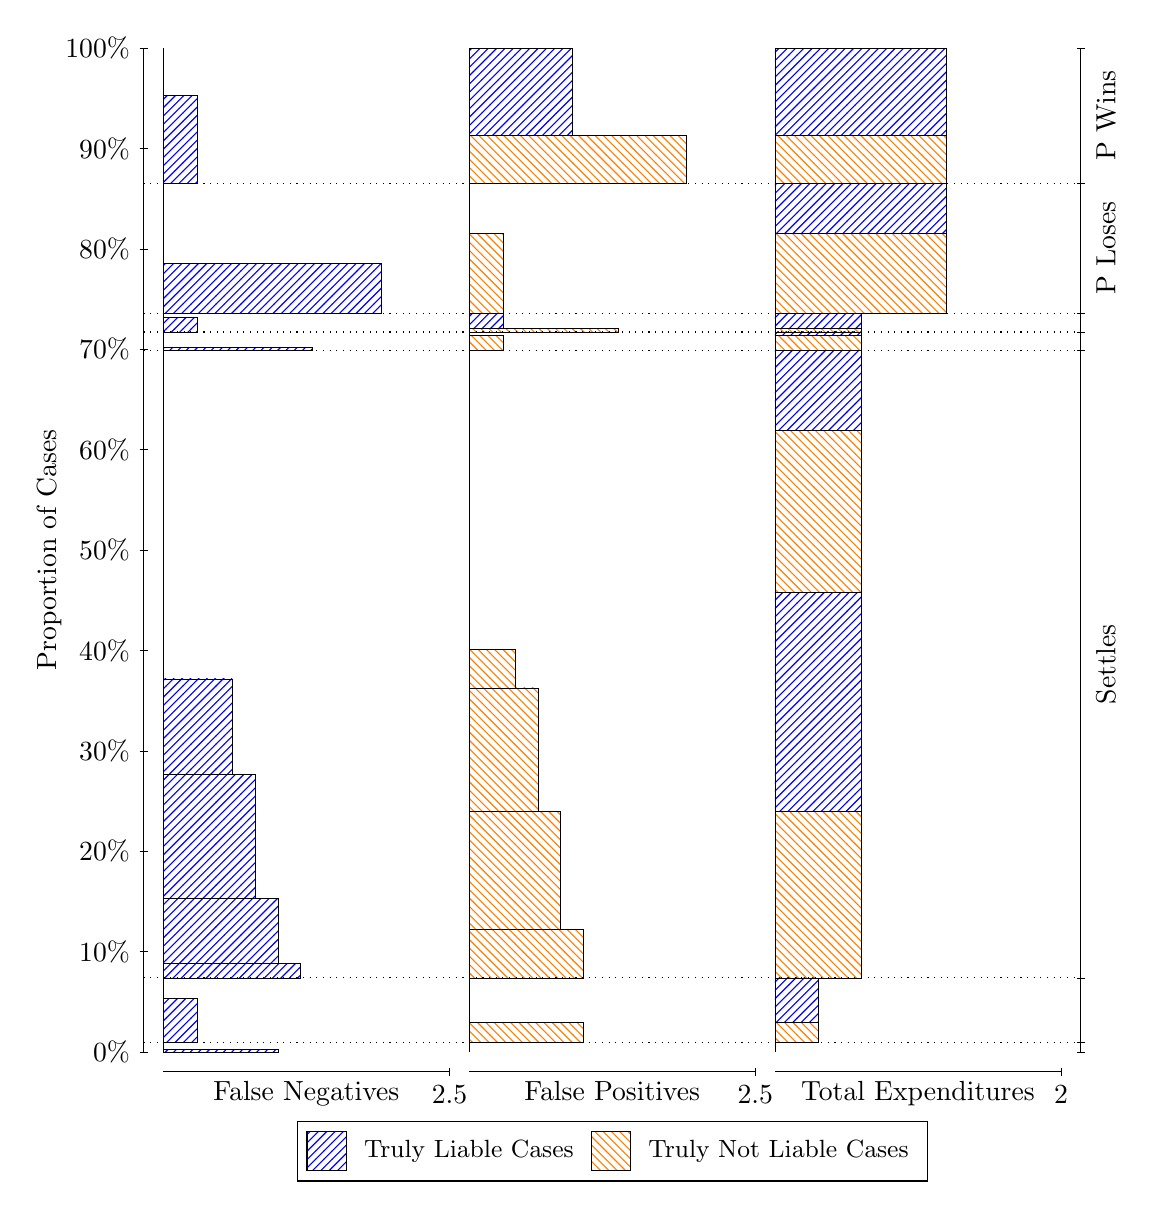
\begin{tikzpicture}
\draw[black, very thin] (1.5,1.75) -- (1.5,14.5);
\node[rotate=90, text=black, anchor=center] at (0.3, 8.125) {Proportion of Cases};
\draw[black, very thin] (1.45,1.75) -- (1.55,1.75);
\node[text=black, anchor=east] at (1.45, 1.75) {0\%};
\draw[black, very thin] (1.45,3.025) -- (1.55,3.025);
\node[text=black, anchor=east] at (1.45, 3.025) {10\%};
\draw[black, very thin] (1.45,4.3) -- (1.55,4.3);
\node[text=black, anchor=east] at (1.45, 4.3) {20\%};
\draw[black, very thin] (1.45,5.575) -- (1.55,5.575);
\node[text=black, anchor=east] at (1.45, 5.575) {30\%};
\draw[black, very thin] (1.45,6.85) -- (1.55,6.85);
\node[text=black, anchor=east] at (1.45, 6.85) {40\%};
\draw[black, very thin] (1.45,8.125) -- (1.55,8.125);
\node[text=black, anchor=east] at (1.45, 8.125) {50\%};
\draw[black, very thin] (1.45,9.4) -- (1.55,9.4);
\node[text=black, anchor=east] at (1.45, 9.4) {60\%};
\draw[black, very thin] (1.45,10.675) -- (1.55,10.675);
\node[text=black, anchor=east] at (1.45, 10.675) {70\%};
\draw[black, very thin] (1.45,11.95) -- (1.55,11.95);
\node[text=black, anchor=east] at (1.45, 11.95) {80\%};
\draw[black, very thin] (1.45,13.225) -- (1.55,13.225);
\node[text=black, anchor=east] at (1.45, 13.225) {90\%};
\draw[black, very thin] (1.45,14.5) -- (1.55,14.5);
\node[text=black, anchor=east] at (1.45, 14.5) {100\%};

\draw[black, very thin] (13.4,1.75) -- (13.4,14.5);
\draw[black, very thin] (13.35,1.75) -- (13.45,1.75);
\node[anchor=west] at (13.35, 1.75) {};
\draw[black, very thin] (13.35,1.8737) -- (13.45,1.8737);
\node[anchor=west] at (13.35, 1.8737) {};
\draw[black, very thin] (13.35,2.6902) -- (13.45,2.6902);
\node[anchor=west] at (13.35, 2.6902) {};
\draw[black, very thin] (13.35,10.657) -- (13.45,10.657);
\node[anchor=west] at (13.35, 10.657) {};
\draw[black, very thin] (13.35,10.894) -- (13.45,10.894);
\node[anchor=west] at (13.35, 10.894) {};
\draw[black, very thin] (13.35,11.131) -- (13.45,11.131);
\node[anchor=west] at (13.35, 11.131) {};
\draw[black, very thin] (13.35,12.785) -- (13.45,12.785);
\node[anchor=west] at (13.35, 12.785) {};
\draw[black, very thin] (13.35,14.5) -- (13.45,14.5);
\node[anchor=west] at (13.35, 14.5) {};

\draw[black, very thin, pattern color=blue, pattern=north east lines] (1.75,1.75) rectangle (3.2033,1.7839);
\draw[black, very thin, pattern color=orange, pattern=north west lines] (1.75,1.7839) rectangle (1.75,1.8737);
\draw[black, very thin, pattern color=blue, pattern=north east lines] (1.75,1.8737) rectangle (2.186,2.4346);
\draw[black, very thin, pattern color=orange, pattern=north west lines] (1.75,2.4346) rectangle (1.75,2.6902);
\draw[black, very thin, pattern color=blue, pattern=north east lines] (1.75,2.6902) rectangle (3.494,2.8768);
\draw[black, very thin, pattern color=blue, pattern=north east lines] (1.75,2.8768) rectangle (3.2033,3.7052);
\draw[black, very thin, pattern color=blue, pattern=north east lines] (1.75,3.7052) rectangle (2.9127,5.278);
\draw[black, very thin, pattern color=blue, pattern=north east lines] (1.75,5.278) rectangle (2.622,6.488);
\draw[black, very thin, pattern color=orange, pattern=north west lines] (1.75,6.488) rectangle (1.75,10.657);
\draw[black, very thin, pattern color=blue, pattern=north east lines] (1.75,10.657) rectangle (3.6393,10.703);
\draw[black, very thin, pattern color=orange, pattern=north west lines] (1.75,10.703) rectangle (1.75,10.894);
\draw[black, very thin, pattern color=blue, pattern=north east lines] (1.75,10.894) rectangle (2.186,11.084);
\draw[black, very thin, pattern color=orange, pattern=north west lines] (1.75,11.084) rectangle (1.75,11.131);
\draw[black, very thin, pattern color=blue, pattern=north east lines] (1.75,11.131) rectangle (4.5113,11.766);
\draw[black, very thin, pattern color=orange, pattern=north west lines] (1.75,11.766) rectangle (1.75,12.785);
\draw[black, very thin, pattern color=blue, pattern=north east lines] (1.75,12.785) rectangle (2.186,13.894);
\draw[black, very thin, pattern color=orange, pattern=north west lines] (1.75,13.894) rectangle (1.75,14.5);
\draw[black, very thin, pattern color=orange, pattern=north west lines] (5.6333,1.75) rectangle (5.6333,1.8397);
\draw[black, very thin, pattern color=blue, pattern=north east lines] (5.6333,1.8397) rectangle (5.6333,1.8737);
\draw[black, very thin, pattern color=orange, pattern=north west lines] (5.6333,1.8737) rectangle (7.0867,2.1292);
\draw[black, very thin, pattern color=blue, pattern=north east lines] (5.6333,2.1292) rectangle (5.6333,2.6902);
\draw[black, very thin, pattern color=orange, pattern=north west lines] (5.6333,2.6902) rectangle (7.0867,3.302);
\draw[black, very thin, pattern color=orange, pattern=north west lines] (5.6333,3.302) rectangle (6.796,4.8034);
\draw[black, very thin, pattern color=orange, pattern=north west lines] (5.6333,4.8034) rectangle (6.5053,6.3727);
\draw[black, very thin, pattern color=orange, pattern=north west lines] (5.6333,6.3727) rectangle (6.2147,6.859);
\draw[black, very thin, pattern color=blue, pattern=north east lines] (5.6333,6.859) rectangle (5.6333,10.657);
\draw[black, very thin, pattern color=orange, pattern=north west lines] (5.6333,10.657) rectangle (6.0693,10.847);
\draw[black, very thin, pattern color=blue, pattern=north east lines] (5.6333,10.847) rectangle (5.6333,10.894);
\draw[black, very thin, pattern color=orange, pattern=north west lines] (5.6333,10.894) rectangle (7.5227,10.94);
\draw[black, very thin, pattern color=blue, pattern=north east lines] (5.6333,10.94) rectangle (6.0693,11.131);
\draw[black, very thin, pattern color=orange, pattern=north west lines] (5.6333,11.131) rectangle (6.0693,12.149);
\draw[black, very thin, pattern color=blue, pattern=north east lines] (5.6333,12.149) rectangle (5.6333,12.785);
\draw[black, very thin, pattern color=orange, pattern=north west lines] (5.6333,12.785) rectangle (8.3947,13.39);
\draw[black, very thin, pattern color=blue, pattern=north east lines] (5.6333,13.39) rectangle (6.9413,14.5);
\draw[black, very thin, pattern color=orange, pattern=north west lines] (9.5167,1.75) rectangle (9.5167,1.8397);
\draw[black, very thin, pattern color=blue, pattern=north east lines] (9.5167,1.8397) rectangle (9.5167,1.8737);
\draw[black, very thin, pattern color=orange, pattern=north west lines] (9.5167,1.8737) rectangle (10.062,2.1292);
\draw[black, very thin, pattern color=blue, pattern=north east lines] (9.5167,2.1292) rectangle (10.062,2.6902);
\draw[black, very thin, pattern color=orange, pattern=north west lines] (9.5167,2.6902) rectangle (10.607,4.8034);
\draw[black, very thin, pattern color=blue, pattern=north east lines] (9.5167,4.8034) rectangle (10.607,7.5862);
\draw[black, very thin, pattern color=orange, pattern=north west lines] (9.5167,7.5862) rectangle (10.607,9.6418);
\draw[black, very thin, pattern color=blue, pattern=north east lines] (9.5167,9.6418) rectangle (10.607,10.657);
\draw[black, very thin, pattern color=orange, pattern=north west lines] (9.5167,10.657) rectangle (10.607,10.847);
\draw[black, very thin, pattern color=blue, pattern=north east lines] (9.5167,10.847) rectangle (10.607,10.894);
\draw[black, very thin, pattern color=orange, pattern=north west lines] (9.5167,10.894) rectangle (10.607,10.94);
\draw[black, very thin, pattern color=blue, pattern=north east lines] (9.5167,10.94) rectangle (10.607,11.131);
\draw[black, very thin, pattern color=orange, pattern=north west lines] (9.5167,11.131) rectangle (11.697,12.149);
\draw[black, very thin, pattern color=blue, pattern=north east lines] (9.5167,12.149) rectangle (11.697,12.785);
\draw[black, very thin, pattern color=orange, pattern=north west lines] (9.5167,12.785) rectangle (11.697,13.39);
\draw[black, very thin, pattern color=blue, pattern=north east lines] (9.5167,13.39) rectangle (11.697,14.5);
\draw[black, dotted] (1.5,1.8737) -- (13.4,1.8737);
\draw[black, dotted] (1.5,2.6902) -- (13.4,2.6902);
\draw[black, dotted] (1.5,10.657) -- (13.4,10.657);
\draw[black, dotted] (1.5,10.894) -- (13.4,10.894);
\draw[black, dotted] (1.5,11.131) -- (13.4,11.131);
\draw[black, dotted] (1.5,12.785) -- (13.4,12.785);
\draw[black, very thin] (1.75,1.5) -- (5.3833,1.5);
\node[text=black, anchor=north] at (3.5667, 1.5) {False Negatives};
\draw[black, very thin] (5.3833,1.45) -- (5.3833,1.55);
\node[text=black, anchor=north] at (5.3833, 1.45) {2.5};

\draw[black, very thin] (5.6333,1.5) -- (9.2667,1.5);
\node[text=black, anchor=north] at (7.45, 1.5) {False Positives};
\draw[black, very thin] (9.2667,1.45) -- (9.2667,1.55);
\node[text=black, anchor=north] at (9.2667, 1.45) {2.5};

\draw[black, very thin] (9.5167,1.5) -- (13.15,1.5);
\node[text=black, anchor=north] at (11.333, 1.5) {Total Expenditures};
\draw[black, very thin] (13.15,1.45) -- (13.15,1.55);
\node[text=black, anchor=north] at (13.15, 1.45) {2};



\node[text=black, centered, rotate=90] at (13.72, 6.6735) {Settles};


\node[text=black, centered, rotate=90] at (13.72, 11.958) {P Loses};
\node[text=black, centered, rotate=90] at (13.72, 13.642) {P Wins};

\draw (7.449999999999999,1.5) node[draw=none] (baseCoordinate) {};
\begin{scope}[align=center]
        \matrix[scale=0.5, draw=black, below=0.5cm of baseCoordinate, nodes={draw}, column sep=0.1cm]{
            \node[rectangle, draw, minimum width=0.5cm, minimum height=0.5cm, pattern color=blue, pattern=north east lines] {}; &
            \node[draw=none, font=\small, text=black] (B) {Truly Liable Cases}; &
            \node[rectangle, draw, minimum width=0.5cm, minimum height=0.5cm, pattern color=orange, pattern=north west lines] {}; &
            \node[draw=none, font=\small, text=black] (B) {Truly Not Liable Cases}; \\
            };
\end{scope}

\end{tikzpicture}
\end{document}